\section{Input \& Output}

\begin{multicols}{2}

\begin{figure}[H]
    \centering
    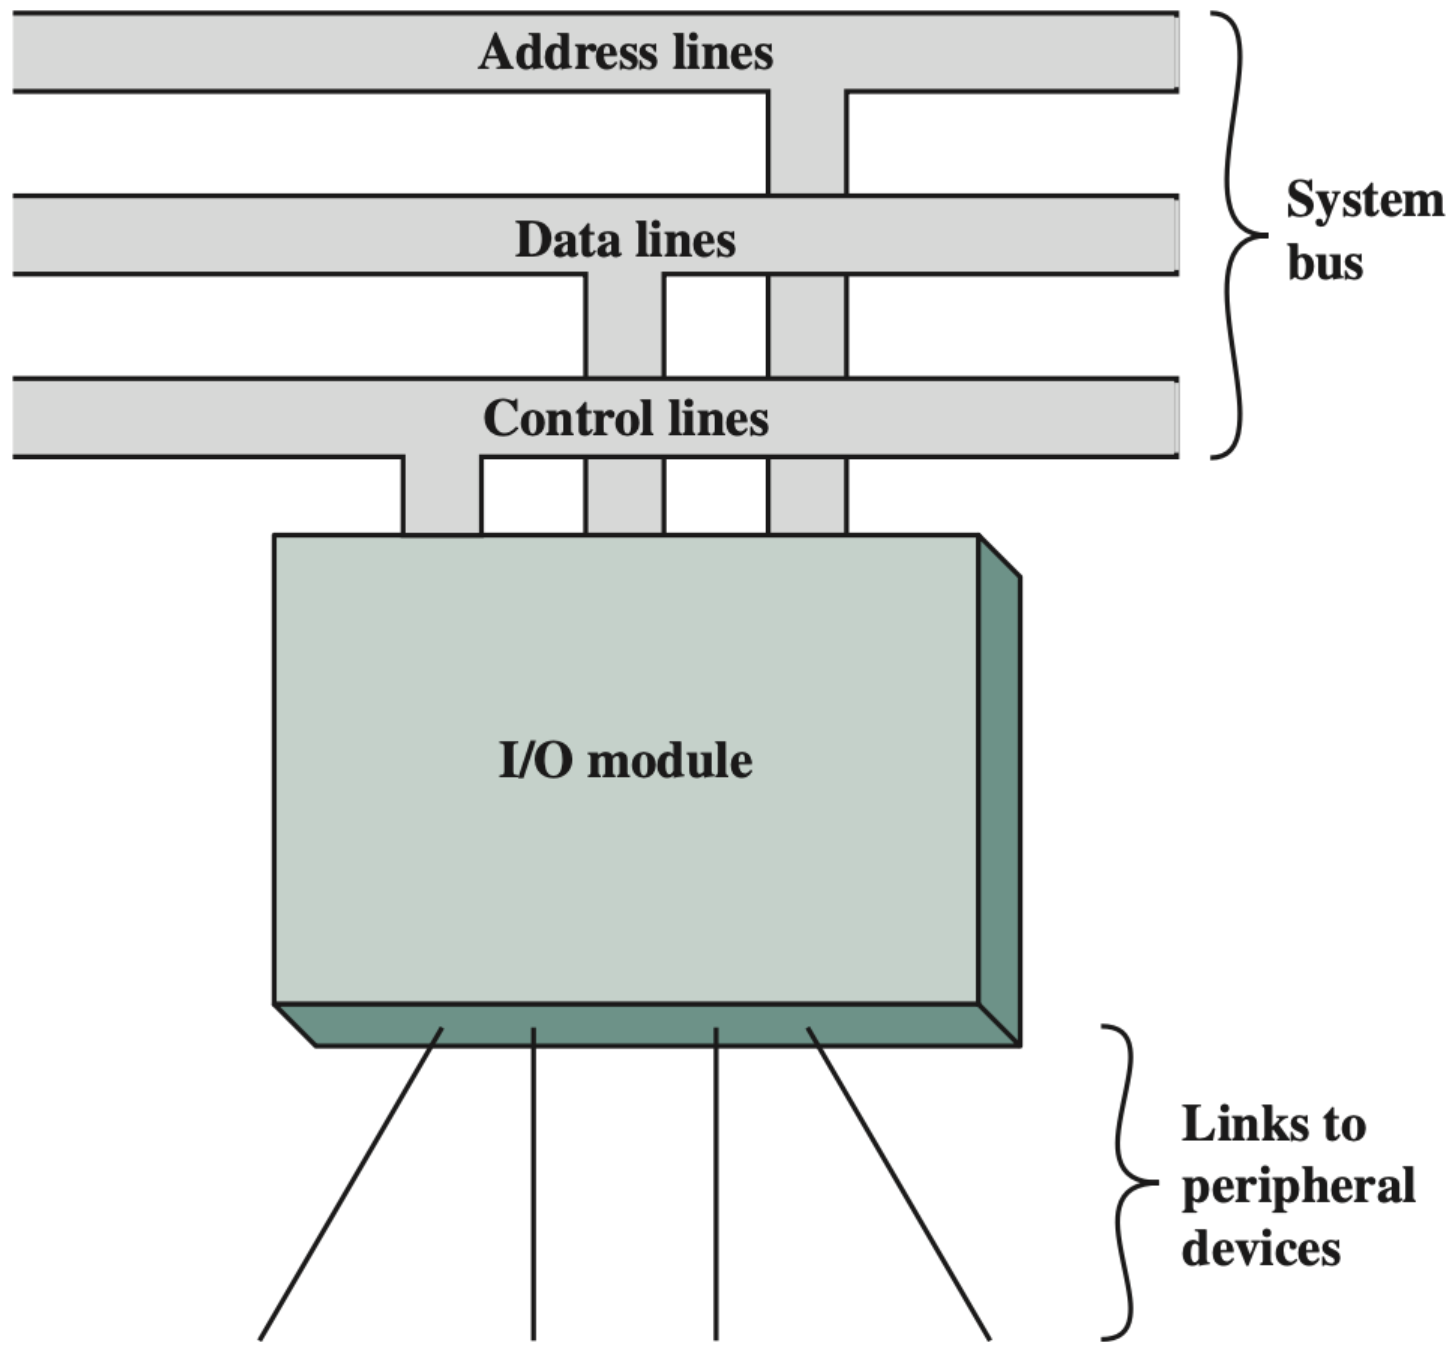
\includegraphics[width=\linewidth]{chaps/input-output/io-module-model.png}
    \caption{Generic Model of an I/O Module}
\end{figure}

\columnbreak

\subsection{Generic Model of I/O Modules}

An I/O module is:
\begin{itemize}
    \item an interface between the processor and memory via the system bus or central switch
    \item an interface to one ore more peripheral devices through tailored data links
\end{itemize}

Major requirements on an I/O module:
\begin{itemize}
    \item \textbf{Asynchronous timing}.
    \item \textbf{Command decoding}: interpret the commands sent from the bus, e.g. \texttt{SEEK}.
    \item \textbf{Data}: exchange data via the data bus.
    \item \textbf{Status reporting}: e.g. Ready, Busy, Out of Paper (printer).
    \item \textbf{Address recognition}: identify the address of a peripheral device.
    \item \textbf{Data buffering}: for speeding up transaction because the device may be slower.
    \item \textbf{Error detection and correction}.
\end{itemize}

\end{multicols}

The CPU operates I/O devices by reading/writing from/to the devices' status/control/data
registers. The registers are mapped in two ways:
\begin{enumerate}
    \item \textbf{Memory-mapped I/O}: the I/O device registers are mapped into the same
        address space as the memory. The CPU can access the I/O device registers as if
        they were memory locations.
    \item \textbf{Port-mapped I/O}: the I/O device registers are mapped into a separate
        address space from the memory. The CPU uses special I/O instructions to access
        the I/O device registers.
\end{enumerate}